\documentclass{article} % For LaTeX2e
\usepackage{nips14submit_e,times}
\usepackage{amsmath}
\usepackage{amsthm}
\usepackage{amssymb}
\usepackage{mathtools}
\usepackage{hyperref}
\usepackage{url}
\usepackage{algorithm}
\usepackage[noend]{algpseudocode}
%\documentstyle[nips14submit_09,times,art10]{article} % For LaTeX 2.09

\usepackage{graphicx}
\usepackage{caption}
\usepackage{subcaption}

\def\eQb#1\eQe{\begin{eqnarray*}#1\end{eqnarray*}}
\def\eQnb#1\eQne{\begin{eqnarray}#1\end{eqnarray}}
\providecommand{\e}[1]{\ensuremath{\times 10^{#1}}}
\providecommand{\pb}[0]{\pagebreak}
\DeclarePairedDelimiter\ceil{\lceil}{\rceil}
\DeclarePairedDelimiter\floor{\lfloor}{\rfloor}

\newcommand{\E}{\mathrm{E}}
\newcommand{\Var}{\mathrm{Var}}
\newcommand{\Cov}{\mathrm{Cov}}

\def\Qb#1\Qe{\begin{question}#1\end{question}}
\def\Sb#1\Se{\begin{solution}#1\end{solution}}

\newenvironment{claim}[1]{\par\noindent\underline{Claim:}\space#1}{}
\newtheoremstyle{quest}{\topsep}{\topsep}{}{}{\bfseries}{}{ }{\thmname{#1}\thmnote{ #3}.}
\theoremstyle{quest}
\newtheorem*{definition}{Definition}
\newtheorem*{theorem}{Theorem}
\newtheorem*{lemma}{Lemma}
\newtheorem*{question}{Question}
\newtheorem*{preposition}{Preposition}
\newtheorem*{exercise}{Exercise}
\newtheorem*{challengeproblem}{Challenge Problem}
\newtheorem*{solution}{Solution}
\newtheorem*{remark}{Remark}
\usepackage{verbatimbox}
\usepackage{listings}
\usepackage{mathrsfs}
\title{DiffGeoI: \\
Problem Set I}


\author{
Youngduck Choi \\
CIMS \\
New York University\\
\texttt{yc1104@nyu.edu} \\
}


% The \author macro works with any number of authors. There are two commands
% used to separate the names and addresses of multiple authors: \And and \AND.
%
% Using \And between authors leaves it to \LaTeX{} to determine where to break
% the lines. Using \AND forces a linebreak at that point. So, if \LaTeX{}
% puts 3 of 4 authors names on the first line, and the last on the second
% line, try using \AND instead of \And before the third author name.

\newcommand{\fix}{\marginpar{FIX}}
\newcommand{\new}{\marginpar{NEW}}

\nipsfinalcopy % Uncomment for camera-ready version

\begin{document}


\maketitle

\begin{abstract}
This work contains solutions to the exercises of the problem set I.
\end{abstract}

\bigskip

\begin{question}[1]
\hfill
\begin{figure}[h!]
  \centering
    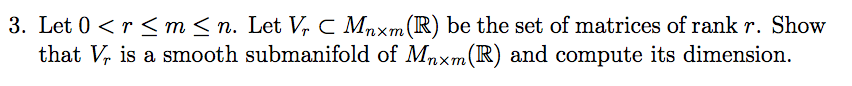
\includegraphics[width=0.7\textwidth]{geo-2-1.png}
\end{figure}
\end{question}
\begin{solution} \hfill \\
Let $M_k(m \times n, \mathbb{R})$ be the subset matrices of rank $k$. 
We claim that it is an embedded submanifold of dimension $mn - (m-k)(n-k)$.
Let $E_0 \in M_k(m \times n, \mathbb{R})$. We write
\eQb
E_0 &=& \begin{pmatrix}
A_0 & B_0 \\
C_0 & D_0 \\
\end{pmatrix},
\eQe
where $A_0$ is non-singular $k\times k$, and $D_0$ is $(m-k) \times (m-k)$.
Define $U$ by
\eQb
U &=& \{\begin{pmatrix} 
A & B \\
C & D \\
\end{pmatrix} \in M(m \times n, \mathbb{R}) \> : \> \det A \neq 0\}. 
\eQe
Since $\det$ is continuous, $U$ is a neighborhood of $E_0$. For any $E 
= \begin{pmatrix} A & B \\ C & D \\ \end{pmatrix} \in U$, set
\eQb
P &=&
\begin{pmatrix} A^{-1} & -A^{-1}B \\ 
0 & I_{n-k} \\
\end{pmatrix}.
\eQe
Observe that $P$ is non-singular, so $EP$ has the same rank as $E$. We compute
\eQb
EP &=& \begin{pmatrix}
I_k & 0 \\
CA^{-1} & D - CA^{-1}B \\
\end{pmatrix},
\eQe 
so $EP$ has rank $r$ iff $D-CA^{-1}B$ is $0$. 
Now, define $\Phi: U \to M((m-k)\times (n-k),\mathbb{R})$ by
\eQb
\Phi \begin{pmatrix}
A & B \\
C & D \\
\end{pmatrix} &=& D - CA^{-1}B. 
\eQe
Consider $D\Phi(E)$. Define a curve $\gamma: \mathbb{R} \to U$ by
\eQb
\lambda(t) &=& \begin{pmatrix}
A & B \\
C & D+tX \\
\end{pmatrix}.
\eQe
We compute
\eQb
\Phi_{*} \gamma^{'}(0) &=& dt_{t=0} (D + tX - CA^{-1}B) = X.
\eQe
Therefore, $\Phi$ is a submersion, which shows that $M_{k}(m \times n , \mathbb{R})
\cap U$ is an embedded submanifold of $U$. Suppose $E_0'$ is any matrix of rank $k$.
Through row-column operations, $R$,  which is linear and preserves rank, $U'$ is a 
neighborhood $E_0'$. Then, for $\Phi \circ R$ is a submersion whose zero set is
$M_k(m \times n , \mathbb{R}) \cap U'$. Therefore, $M_k(m\times n , \mathbb{R})$
is an embedded submanifold. \hfill $\qed$

\end{solution}

\newpage

\begin{question}[2]
\hfill
\begin{figure}[h!]
  \centering
    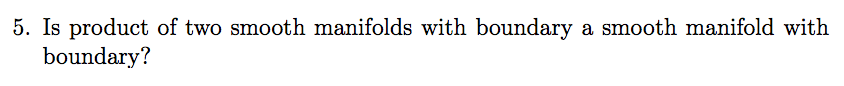
\includegraphics[width=0.7\textwidth]{geo-2-2.png}
\end{figure}
\end{question}
\begin{solution} \hfill \\
It is not true in general. Consider $[0,1]$ with a smooth maximal half-space atlas,
induced by a smooth half-space atlas 
$\{ ([0,\dfrac{2}{3}),x) , ((\dfrac{1}{3},1],1-x)\}$. Now, consider the product
manifold, and choosing the $x$ charts, we see that 
$x \times x ([0,\dfrac{2}{3}) \times [0,\dfrac{2}{3})) = 
[0,\dfrac{2}{3}) \times [0,\dfrac{2}{3})$, which is not open in
$\mathbb{R} \times [0,\infty)$. This violates the fact that the
chart needs to map into an open set, which shows that a product of manifold
with boundaries is not a manifold with boundary. \hfill $\qed$
\end{solution}

\newpage

\begin{question}[3]
\hfill
\begin{figure}[h!]
  \centering
    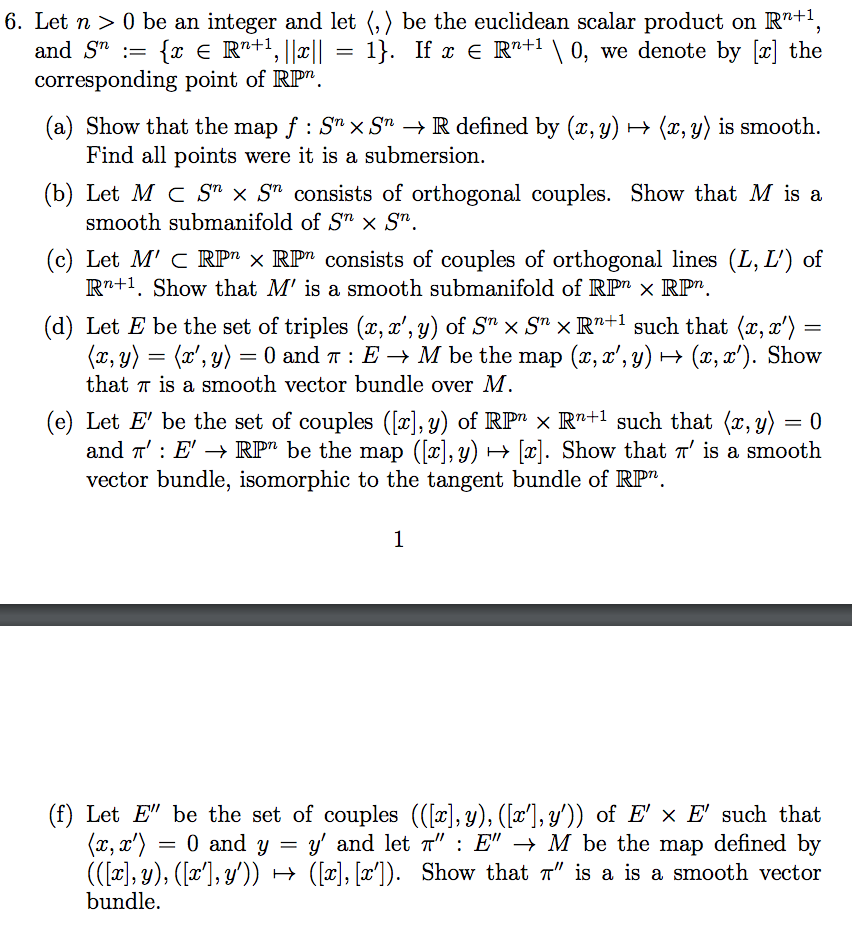
\includegraphics[width=0.7\textwidth]{geo-2-3.png}
\end{figure}
\end{question}
\begin{solution} \hfill \\
 \textbf{(a)} Let $p = (x_1^*,...,x_{n+1}^*,y_1^*,...,y_{n+1}^*) 
\in S^n \times S^n$.
Without loss of generality, suppose that $p \in U_N \times U_N$. Then, we have
the associated projection being $\phi = \psi_N \times \psi_N$, and choose 
$\mathbb{R},id)$ chart for $f(p)$. We aim to show that
\eQb
id \circ f \circ \phi^{-1} = f \circ \phi^{-1}
\eQe 
is smooth. For any $q = (x_1,...,x_{n+1},y_1,...y_{n+1}) \in U_N \times U_N$,
\eQb
\phi(q) &\mapsto
\eQe
 

\textbf{(a)} Let $p = (x_1^*,...,x_n^*,y_1^*,...,y_n^*) \in S^n \times S^n$. 
Without loss of 
generality, suppose that $x_n^*, y_n^* > 0$. 
Choose ${U_{n}}^{+} \times {U_n}^{+}$ with
the associated projection map, $\phi$ 
as the chart for $p$ and choose $(\mathbb{R},id)$. We aim to show that 
$id \circ f \circ \phi^{-1} = f \circ \phi^{-1}$ is smooth. For any $q
= (x_1,...,x_{n},y_1,...,y_n) \in U_{n}^{+}
\times {U_n}^{+}$, 
\eQb
(\phi(q)) \mapsto 
(x_1,...,(1-\sum_{i =1}^{n-1} {x_i}^2)^{\frac{1}{2}}),y_1,...,(1-\sum_{i=1}^{n-1}
{y_i}^2)^{\frac{1}{2}}) \mapsto  \sum_{i=1}^{n-1} x_i y_i + \\ 
(1-\sum_{i=1}^{n-1} {x_i}^2)^{\frac{1}{2}})
(1-\sum_{i=1}^{n-1} {y_i}^2)^{\frac{1}{2}}),
\eQe 
which shows that $f \circ \phi^{-1}$ is smooth, because the domain of the map is
$B_{n}\times B_{n}$, where $B_n$ denotes the $n$ dimensional unit ball, lying
on the $x_1-...-x_n$ plane. 

\smallskip
 
Now, taking the differential of $f$ gives

\bigskip
\textbf{(b)} Let $p \in M$, and suppose without loss of generality, $p \in
U_N \times U_S$ (up to re-ordering). Then, it suffices to show that
\eQb
\psi_N \times \psi_S((U_N \times U_S) \cap M) &=& \psi_N \times \psi_S
(M \setminus
((p_N \times S_{n-1}  \cup S_{n-1} \times p_S)),  
\eQe
where $p_N$ and $p_S$ denote north and south poles,
is a submanifold of
$\psi_N \times \psi_S(U_N \times U_S) = (\mathbb{R}^n \setminus \{0\}) \times
(\mathbb{R}^n \setminus \{0\})$. From $(a)$, it should follow that
$f$ provides the necessary submersion.
 

\bigskip

\textbf{(d)} Suppose $n \geq 2$. We first show that $\pi$ defined is surjective.
Suppose $(x,x') \in M$. Then, since the dimension of $\mathbb{R}^{n+1}$ is larger
than $2$ we can choose a vector $y$ orthogonal to both $x$ and $x'$. It follows
that $(x,x',y) \in E$ such that $\pi((x,x',y)) = (x,x')$. Hence, $\pi$ is surjective.
Now, $\pi$ is by definition smooth, because it is a projection defined on a product 
manifold. One can show the smoothness in both direction by choosing the
same chart around $p$ and taking a product with an arbitrary chart on one side.
So far, $\pi$ is surjective and smooth.
Now, for any $p = (x,x') \in M$, we have
\eQb
\pi^{-1}(p) &=& \{ (x,x',y) \> | \> (x,x') \in M \> \text{and} \> 
<x,y> = <x',y> = 0\}.
\eQe
This clearly has a structure of linear space of dimension $n-1$. Take $\{x,x'\}$
as a two linearly independent vectors
of $\mathbb{R}^{n+1}$ and complete it to obtain $A = \{y_1,...,y_{n-1}\}$,
where these are basis elements, excluding $\{x,x'\}$.
Now, an identity map from $span(A)$ to $\pi^{-1}(p)$ is a linear isomorphism.
Pick $p \in M$ and  without loss of genearlity suppose $p \in U_s \times U_s \cap
M$. Then, define
\eQb
\phi: 
\pi^{-1}((U_s \times U_s) \cap M) \to ((U_s \times U_s) \cap M) 
\times \mathbb{R}^{n-1},
\eQe
by 
\eQb
(x,x',y) \in \pi^{-1}((U_s \times U_s) \cap M) &\mapsto& (x,x',\alpha_1,...,\alpha_{n-1}), 
\eQe
where the $\alpha_1,...,\alpha_{n-1}$ are the coefficients of the basis representation
of $\{x,x',y_1,...y_{n-1}\}$, restricted to the $\{y_1,...y_n\}$ part.
The restriction to a point is clearly a vector space isomorphism by the above
discussion. It remains to show that $\phi$ defined is fiber-preserving. 
We compute, for $p = (x,x',y) \in (U_s \times U_s) \cap M$, 
\eQb
\phi(\pi^{-1}(p)) = \phi(\pi^{-1}(x,x',y)) = \phi((x,x')\times \mathbb{R}^{n+1})
\subset (x,x')\times \mathbb{R}^{n-1} = \pi'^{-1}(p), 
\eQe
where $\pi'$ is the induced differomorphism for the diagram.
It also follows that $\phi$ is a differomorphism as above, and we are done.

\bigskip

\textbf{(e)} Analogous to $(d)$, $\pi^{'}$ is surjective and smooth. Fix $p = [x] \in 
\mathbb{RP}$. Then,
\eQb
\pi'^{-1}(p) &=& \{ ([x],y) \in \mathbb{RP}^n\times
\mathbb{R}^{n+1} \>\>| \>\> <x,y> = 0 \}.
\eQe
By considering the same construction as $(d)$, it shows that the considered
fiber is isomorphic to $\mathbb{R}^{n}$. In fact, by considering the $\phi$,
but with completed basis $\{x,y_1,...,y_n\}$ from $\{x\}$, shows that $\pi'$
is a vector bundle. 

\bigskip

\textbf{(f)} Analogous to $(d)$, $\pi^{''}$ is surjective and smooth. Note 
that $M$ should be $M'$. Fix $p = ([x],[x']) \in \mathbb{RP}^{n} \times 
\mathbb{RP}^{n}$. Then,
\eQb
\pi''^{-1}([x],[x']) &=& \{ (([x],y),([x'],y') \> | \> <x,x'> = <x,y> = <x',y'> = 0
\>\>\> y = y'\}.
\eQe
By considering the same construction as above, the fiber is isomorphic to
$\mathbb{R}^{n-1} \times \mathbb{R}^{n-1}$. Take $x,x'$ as two linearly independent
and then complete the basis. Since $y=y'$ condition holds, we will have
the isomorphism with the product of $\mathbb{R}^{n-1}\times \mathbb{R}^{n-1}$.
\hfill $\qed$
 
\end{solution}

\end{document}
